\chapter{Applications}
\begin{figure}[h]
  \centering
  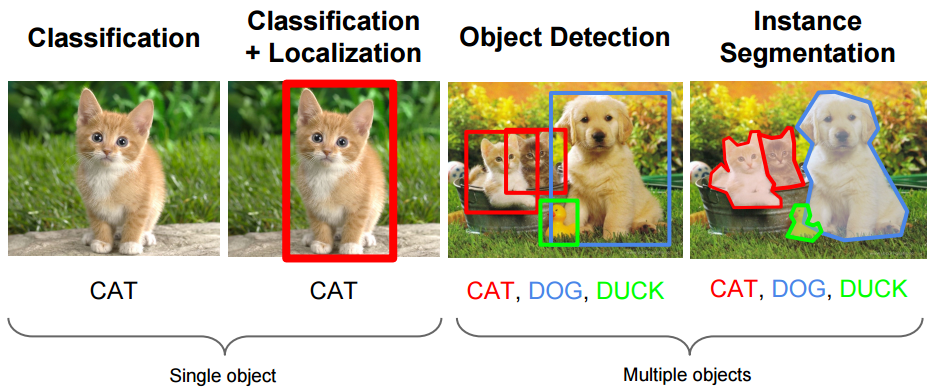
\includegraphics[width=0.55\textwidth]{Images/applications/1.png}
  \caption{Some applications examples}
\end{figure}

\section{Classification}
Train a classification model with softmax loss. The input is the entire image and the output are C probabilities (one per class) of being in the image.
\begin{figure}[h]
  \centering
  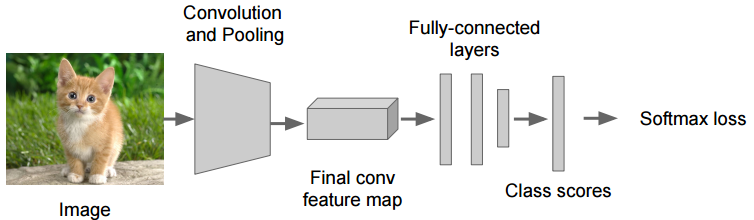
\includegraphics[width=0.55\textwidth]{Images/applications/2.png}
  \caption{Classification}
\end{figure}


\section{Classification + Localization}
Goal is to find a fixed number of objects (one or many) in an image

3 easy steps recipe:

\begin{figure}[h]
  \centering
  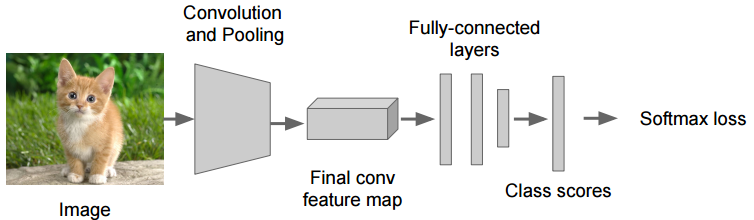
\includegraphics[width=0.55\textwidth]{Images/applications/3.png}
  \caption{1.- Train (or download) a classification model (AlexNet, VGG, GoogLeNet)}
\end{figure}
\begin{figure}[h]
  \centering
  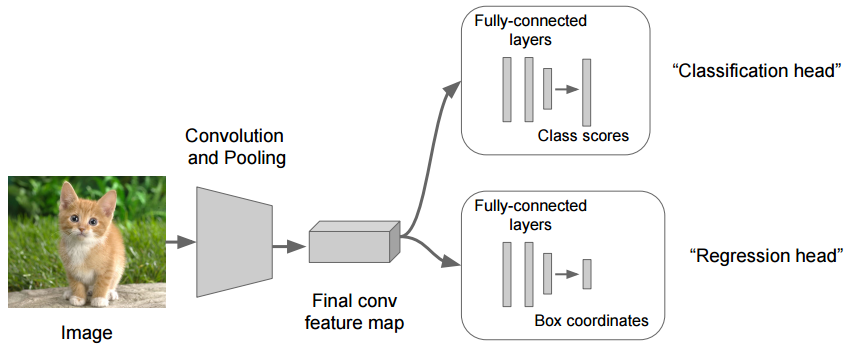
\includegraphics[width=0.55\textwidth]{Images/applications/26.png}
  \caption{2.- Attach a new fully-connected "regression head" to the network to compute bounding boxes (x,y,w,h)}
\end{figure}

\begin{figure}[h]
  \centering
  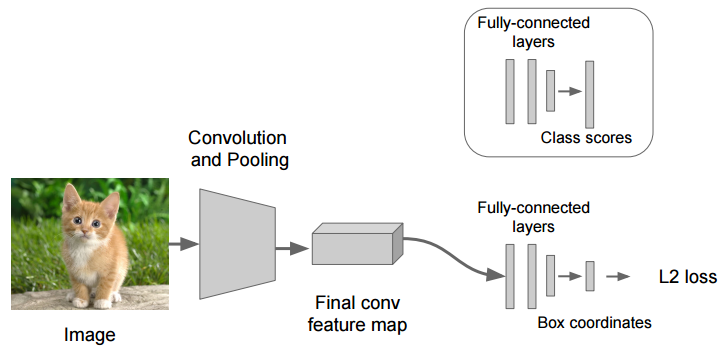
\includegraphics[width=0.55\textwidth]{Images/applications/4.png}
  \caption{3.- Train the regression head only with SGD and L2 loss with the bounding boxes as ground-truth.}
\end{figure}


When training the regression head there are two options: You can backpropagate only till the regression head or the entire network. 2nd option will improve a little bit the accuracy at a expense of higher training computation cost. If you choose option 2 you will be changing the original Conv layers on which the classification head is trained. So there are two options. Or you have two independent networks: the original one (Conv+classification head) and the other one (Modified Conv+regression head). Or you train both at the same time so you will have only one model(classification head + regression head).

\begin{figure}[h]
  \centering
  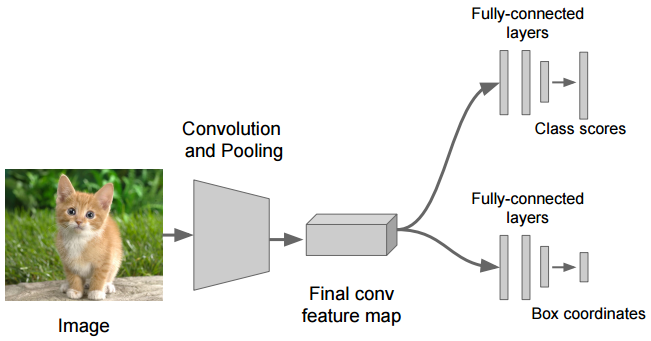
\includegraphics[width=0.55\textwidth]{Images/applications/5.png}
  \caption{4.- At test time use both heads}
\end{figure}


The final DNN for classification + uses both heads at test time
\begin{itemize}
\item Classification head:
\item The output are $C$ numbers (one per class)
\item Regression head:
\item There are two regression heads strategies (choose one):
\begin{enumerate}
    \item Class agnostic: Output 4 numbers (one bounding box)
    \item Class specific: Output $C \times 4$ numbers (one bounding box per class)
\end{enumerate}
\end{itemize}

Notice that instead of training a regression head which outputs bounding boxes, we could have train it to output a specific number of joints or whatever

\subsection*{Sliding windows (DO NOT DO THIS)}
At test time this (classification + regression) network should be applied inside a sliding windows at multiple scales. (This would have an \textbf{enormous computation cost}, we will see later that there is a better way of doing this).

\begin{figure}[h]
  \centering
  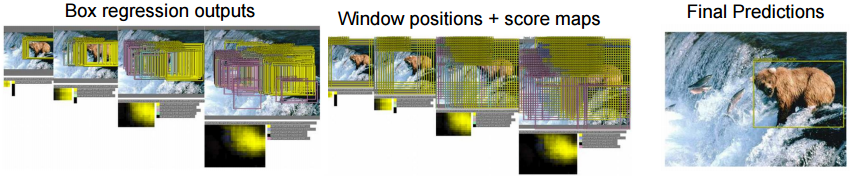
\includegraphics[width=0.55\textwidth]{Images/applications/28.png}
  \caption{Classification + Localization - Box regression and Sliding windows diagram}
\end{figure}

The idea is to run the classification + regression network inside a sliding windows and at multiple scales. So for each windows position we obtain a cat bb (x,y,w,h) and the probability of a cat being inside the current sliding windows position. (This would have an enormous computation cost, we will see later that there is a better way of doing this)

Finally, we have obtained multiple bound boxes and we must merge them and estimate the prob of this final bb of containing a cat. To do so, an algorithm such us non-max suppression could be used.

\subsection*{Bounding Box regression (ONLY INPUT IMAGE FIXED SIZE)}
\begin{figure}[h]
  \centering
  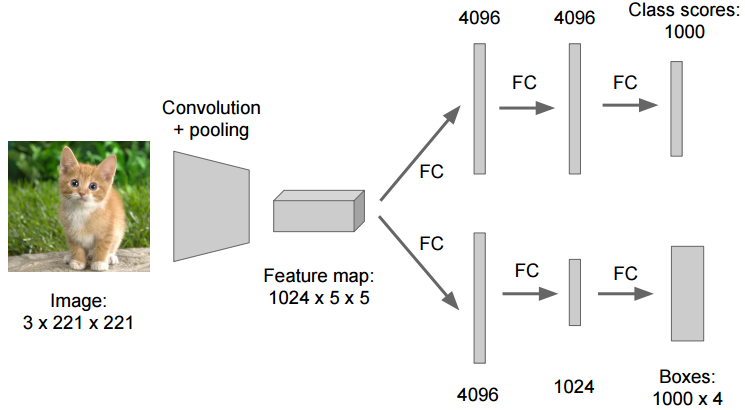
\includegraphics[width=0.45\textwidth]{Images/applications/8.png}
  \caption{Classification + Localization - Box regression architecture}
\end{figure}

Fully connected layers can only deal with input of a fixed size, because it requires a certain amount of parameters to "fully connect" the input and output.

In the example network with fully-connected layers at the end, a $221*221$ image will output a 1000 size vector of class scores. If we apply the network on a larger image, the network will fail because of the inconsistency between the input and parameters of the first fully-connected layer.

In other words, we would have to execute the DNN in each sliding windows position. This has an enormous computation cost. To solve this we can transform the FC layers to Conv layers. (see right column)

\subsection*{Without sliding windows (DO THIS)}

Any FC layer can be converted to a CONV layer. For example, in this model, the FC layer with K=4096 that is looking at the input volume of size $5 \times 5 \times 1024$ can be equivalently expressed as a CONV layer with $F=5,P=0,S=1,K=4096$.

In other words, we are setting the filter size to be exactly the size of the input volume, and hence the output will simply be $1 \times 1 \times 4096$ since only a single depth column ``fits" across the input volume, giving identical result as the initial FC layer.

\begin{figure}[h]
  \centering
  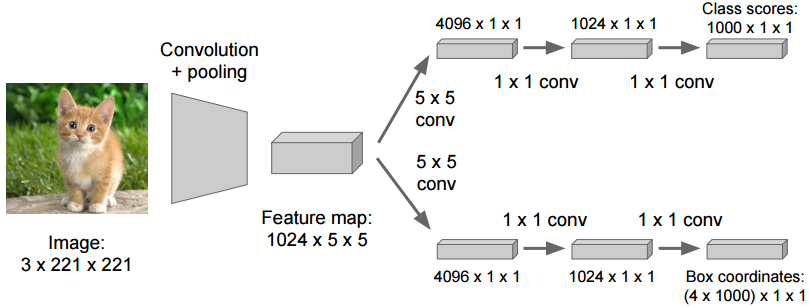
\includegraphics[width=0.55\textwidth]{Images/applications/9.png}
  \caption{Classification + Localization - Without sliding windows}
\end{figure}

FC can only deal with input of a fixed size, while convolutional layers just "slide" the same filters across the input, so it can basically deal with input of an arbitrary spatial size.

\begin{figure}[h]
  \centering
  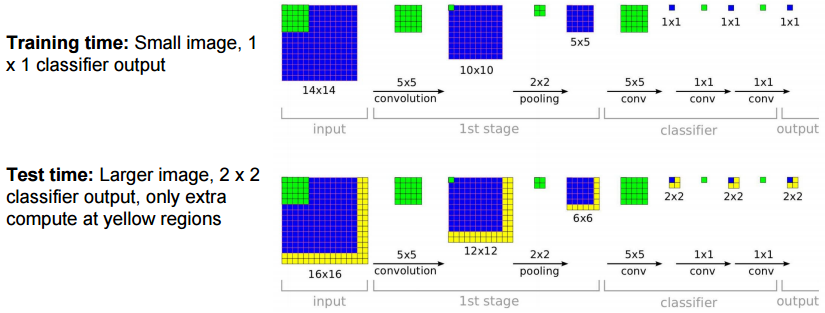
\includegraphics[width=0.7\textwidth]{Images/applications/10.png}
  \caption{ConvLayers allow input of any size in an efficient way}
\end{figure}

At train time we train with samples of the sliding windows. At test time we can evaluate input images of higher dimension sharing computations.

For example, in this image, we have trained the model with input image sizes of $14 \times 14$ producing and output vector of $1 \times 1 \times C$. At test time, we are using input images of $16 \times 16$ which produces and output of $2 \times 2 \times C$. This is equivalent to execute the model 4 times (in the four corners of the image) like in the previous example of the cat. But instead of doing the whole computation 4 times, we are sharing the computation, the extra computation is only done in the yellow parts.

No more sliding windows!!

\section{Object Detection}
Object detection is a harder problem than classification + localization. Now, there can be a non fix number of instances of the same class as well as other classes. We can not use regression with detection (as within classification) because we need variable sized outputs. So we have to go back to sliding windows? It would be very costly to run a classification model in each windows position. The answer is no. We will first search for tiny subsets of possible positions. This models are called R-CNN (Region based CNN).

\textbf{Evaluation}. To evaluate a detection model we use "mean average precision" (mAP). Compute average precision (AP) separately for each class, then average over classes. A detection is a true positive if it has a loU with a ground-truth box greater than some threshold (usually 0.5) (mAP@0.5). Combine all detection from all test images to draw a precision / recall curve for each class; AP is the area under the curve. mAP is a number from 0 to 100. The higher the better.

There are two main networks used for object detection explained in previous chapters:
\begin{itemize}
\item R-CNN (Region Based CNN) - R-CNN, Fast R-CNN \& Faster R-CNN
\item YOLO (You only look once)
\end{itemize}


\section{Segmentation}
\subsection{Semantic Segmentation}
Semantic Segmentation tries to label every pixel. It does not differentiate instances (e.g. cows are a massive compact blue mass)
\begin{figure}[h]
  \centering
  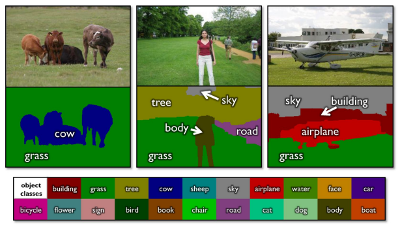
\includegraphics[width=0.6\textwidth]{Images/applications/14.png}
  \caption{Semantic Segmentation}
\end{figure}

\begin{figure}[h]
  \centering
  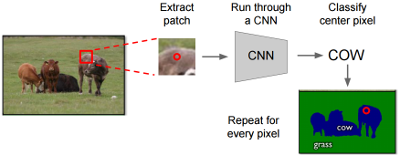
\includegraphics[width=0.6\textwidth]{Images/applications/15.png}
  \caption{General idea. Problem: Smaller output due to pooling. Other more complex solutions are required }
\end{figure}


There are three common strategies used for semantic segmentation:

\begin{itemize}
\item Multiscale, or
\item Refinement, or
\item Upsampling
\end{itemize}

\subsubsection*{Multiscale}

\begin{figure}[h]
  \centering
  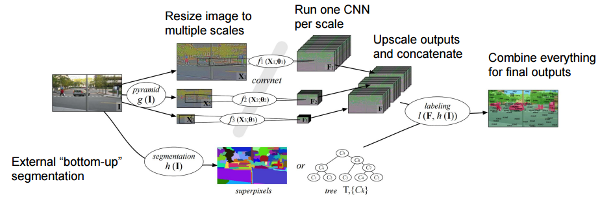
\includegraphics[width=0.65\textwidth]{Images/applications/16.png}
  \caption{Farabet et al,``Learning Hierarchical Features for Scene Labeling", TPAMI 2013}
\end{figure}

Solve problem by working in different scales and up-scaling output. In this example they are also doing a parallel process to compute super-pixels to improve the segmentation.



\subsubsection*{Refinement}
\begin{figure}[h]
  \centering
  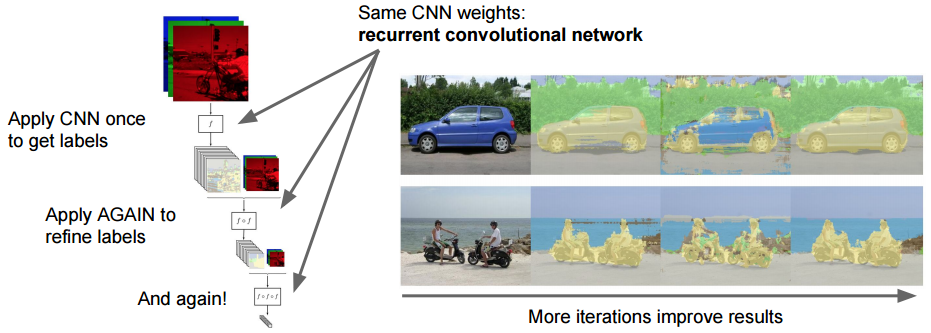
\includegraphics[width=0.65\textwidth]{Images/applications/17.png}
  \caption{Pinheiro and Collobert, ``Recurrent Convolutional Neural Networks for Scene Labeling", ICML 2014}
\end{figure}

\begin{enumerate}
\item Pass the input image through a CNN which produces the low res image segmentation (labels).
\item Rescale the inputs to the lower resolution and apply again the ConvNet to the lower resolution input image and results from the previous segmentation
\item Goto 2 until threshold
\end{enumerate}



\subsubsection*{Upsampling}
\begin{figure}[h]
  \centering
  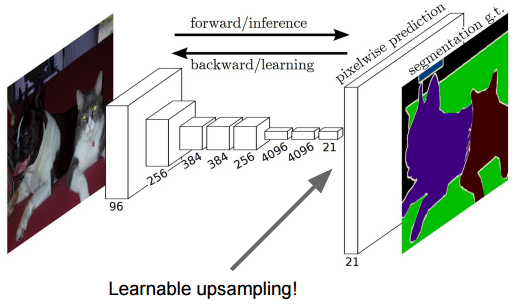
\includegraphics[width=0.5\textwidth]{Images/applications/18.png}
  \caption{Long, Shelhamer, and Darrell, ``Fully Convolutional Networks for Semantic Segmentation", CVPR 2015}
\end{figure}
They pass the input image through a CNN which produces the low res image segmentation (labels). But with this method, they add an extra learnable layer at the end of the ConvNet that learns to upsample the low resolution segmentation (Upsampling layer). The also do skip connections



\subsection{Instance Segmentation}

Detect instances, give category, label pixels. “simultaneous detection and segmentation” (SDS). Normally look very similar to the detection models.

\begin{figure}[h]
  \centering
  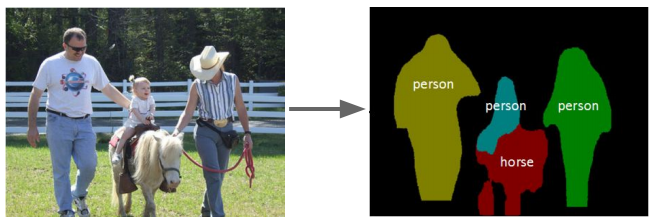
\includegraphics[width=0.5\textwidth]{Images/applications/19.png}
  \caption{Instance Segmentation}
\end{figure}

\subsubsection*{Architecture similar to R-CNN}

\begin{figure}[h]
  \centering
  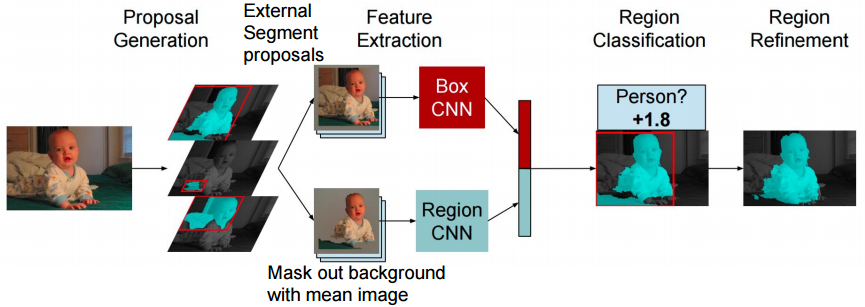
\includegraphics[width=0.6\textwidth]{Images/applications/20.png}
  \caption{Architecture - Hariharan et al, ``Simultaneous Detection and Segmentation", ECCV 2014}
\end{figure}

\begin{enumerate}
\item External segment proposals that outputs pixels not boxes
\item Produce a BBox of the segmented region
\item Take the BBox image an run it through a CNN
\item Take the BBox image and set the non segment proposal pixels to the mean image value of the dataset an run it through a CNN
\item Concatenate booth features an run it through a classifier
\item Refine the proposed region
\end{enumerate}

Notice that this is very similar to R-CNN

For the refinement step there is a following paper that improves it (Hariharan et al, “Hypercolumns for Object Segmentation and Fine-grained Localization”, CVPR 2015). The idea is that once we have the region cropped pass it through AlexNet and extract features of various layers. Then, upsample this feature maps and combine them together. Finally, do a logistic classifier for each of the pixels that predicts how much likely is to be background.

\subsubsection*{Architecture similar to Faster R-CNN}
\begin{figure}[h]
  \centering
  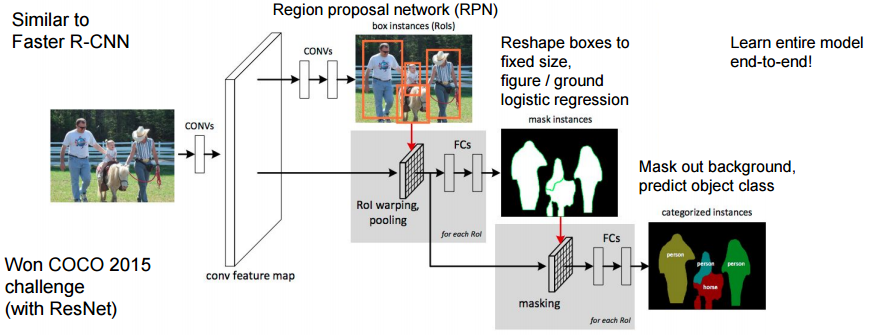
\includegraphics[width=0.6\textwidth]{Images/applications/21.png}
  \caption{Architecture - Dai et al, ``Instance-aware Semantic Segmentation via Multi-task Network Cascades", arXiv 2015}
\end{figure}


Stuck the model in the left to ResNet. Similar to Faster R-CNN

From the high resolution feature map propose regions, then reshape boxes and finally mask background and predict object class.

Notice that the three steps (intermediate levels of the net) can be evaluated with ground-truth.

\section{Image captioning}
\begin{figure}[h]
  \centering
  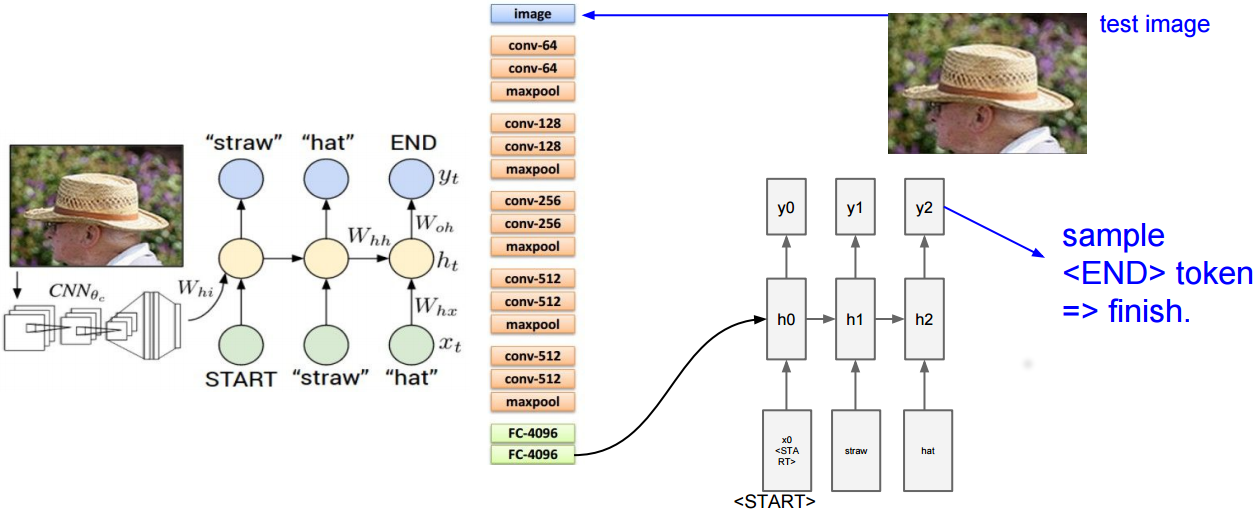
\includegraphics[width=0.65\textwidth]{Images/applications/30.png}
  \caption{``Deep Visual-Semantic Alignments for Generating Image Descriptions", Karpathy and Fei-Fei}
\end{figure}


\section*{Summary}
\begin{itemize}
\item Localization
\begin{itemize}
\item Find a fixed number of objects (one or many)
\item L2 regression from CNN features to box coordinates
\item Overfeat: Regression + efficient sliding window with FC -> conv conversion
\item Deeper networks do better
\end{itemize}
\item Object Detection
\begin{itemize}
\item Find a variable number of objects by classifying image regions
\item Before CNNs: dense multiscale sliding window (HoG, DPM)
\item Avoid dense sliding window with region proposals
\item R-CNN: Selective Search + CNN classification / regression
\item Fast R-CNN: Swap order of convolutions and region extraction
\item Faster R-CNN: Compute region proposals within the network
\item Deeper networks do better
\end{itemize}
\item Semantic segmentation
\begin{itemize}
\item Classify all pixels
\item Fully convolutional models, downsample then upsample
\item Learnable upsampling: fractionally strided convolution
\item Skip connections can help
\end{itemize}
\item Instance Segmentation
\begin{itemize}
\item Detect instance, generate mask
\item Similar pipelines to object detection
\end{itemize}
\end{itemize}